\documentclass{article}

\usepackage{float}
\usepackage{color}
\usepackage{cleveref}
\usepackage{csvsimple}
\usepackage{graphicx}
\usepackage{longtable}
\usepackage{booktabs}
\usepackage{siunitx}

\makeatletter
\newcommand*{\centerfloat}{%
  \parindent \z@
  \leftskip \z@ \@plus 1fil \@minus \textwidth
  \rightskip\leftskip
  \parfillskip \z@skip}
\makeatother

\begin{document}

\begin{table}[H]
    \centering
    \sisetup{round-mode=places, round-precision=2}
    \caption{Average accuracy of all models and data schemes.}
    \csvreader[head to column names,tabular=cccc,
        table head=\toprule \bfseries Model Name & \bfseries Categorization Test & \bfseries Null Test & \bfseries Polarity Test\\\midrule,
        respect underscore=true]{../../results-2/average_centroid_knn.csv}{}
        {\csvcolii  & \num{\csvcoli} & \num{\csvcoliii} & \num{\csvcoliv}}
\end{table}

The following plots compare the centroid and kNN models under variation of the
MFD version (v1 vs v2) and whether duplicate seed words are kept
("share") or removed ("nodups").

\begin{figure}[H]
    \centerfloat
    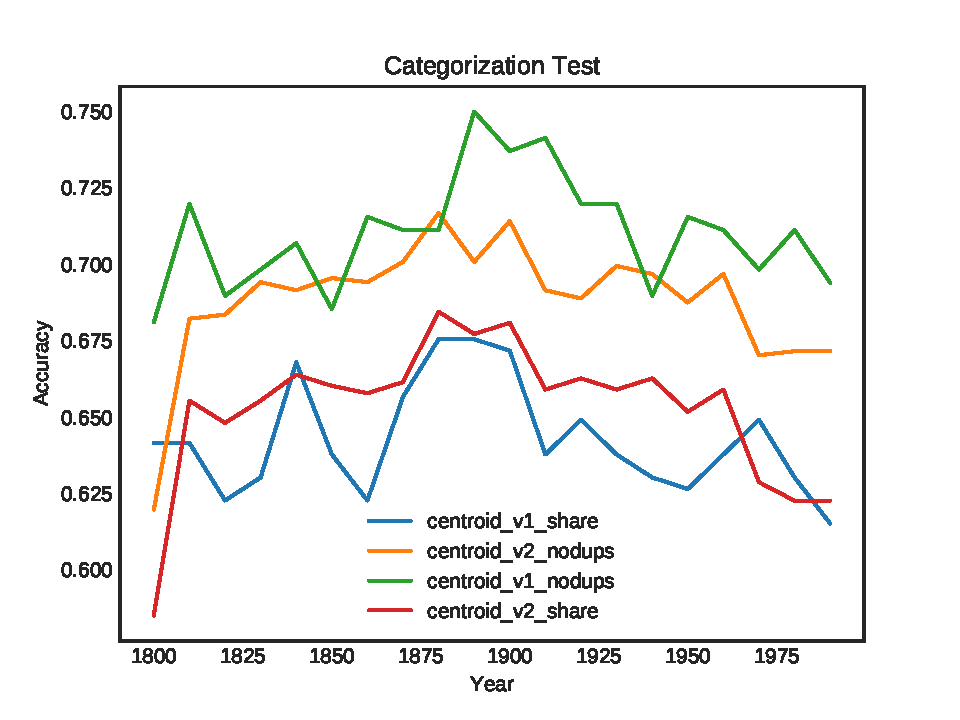
\includegraphics[width=1.3\linewidth]{../../plots-2/centroid/results_categorization_test.pdf}
\end{figure}

\begin{figure}[H]
    \centerfloat
    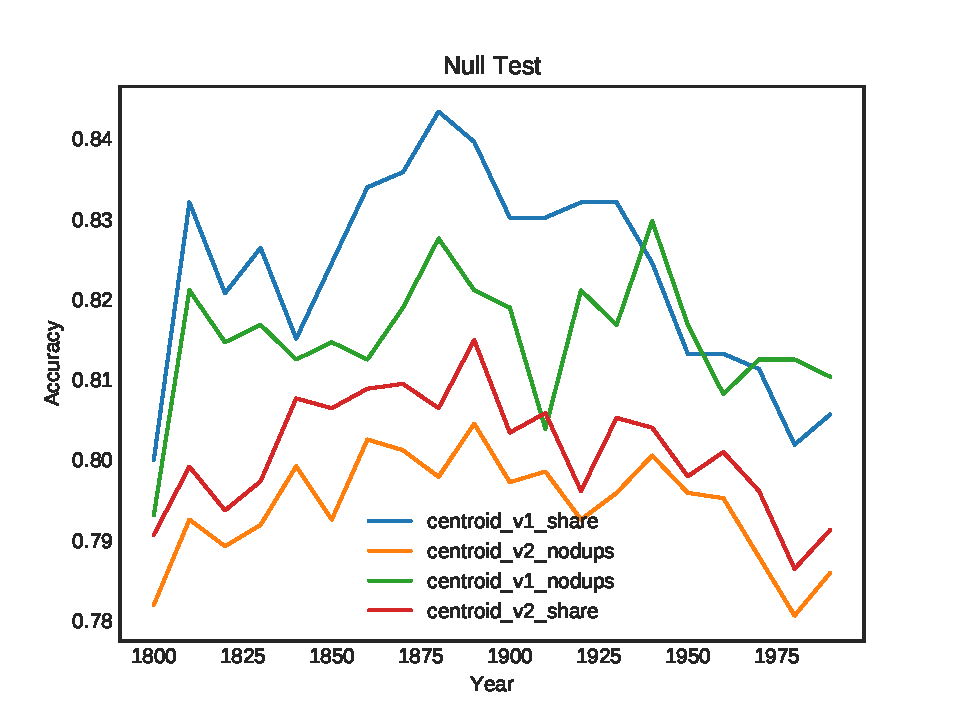
\includegraphics[width=1.3\linewidth]{../../plots-2/centroid/results_null_test.pdf}
\end{figure}

\begin{figure}[H]
    \centerfloat
    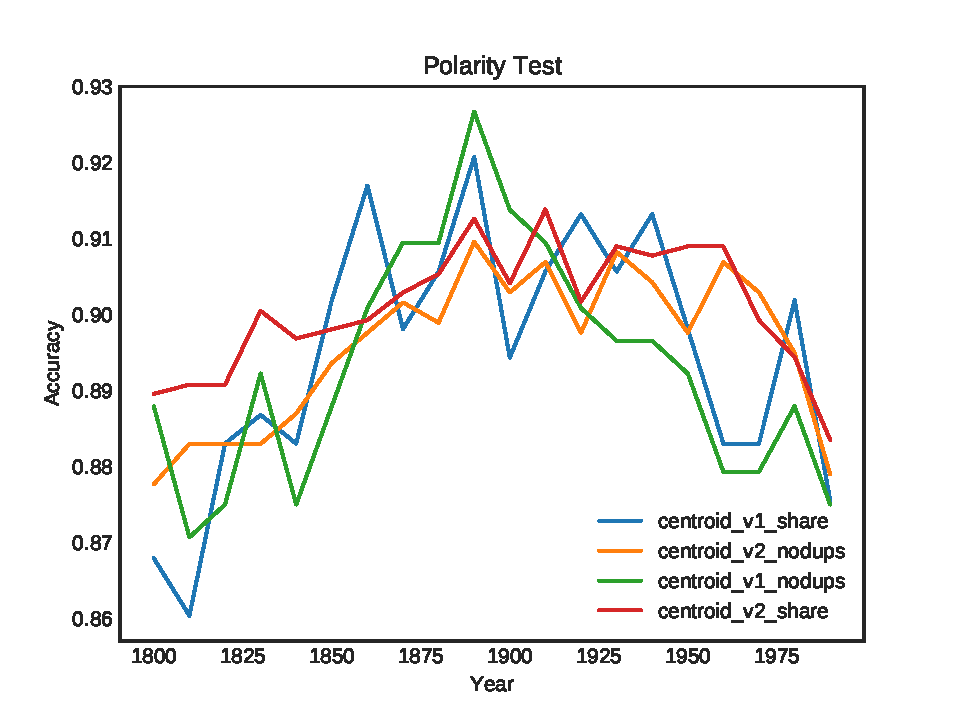
\includegraphics[width=1.3\linewidth]{../../plots-2/centroid/results_polarity_test.pdf}
\end{figure}

\begin{figure}[H]
    \centerfloat
    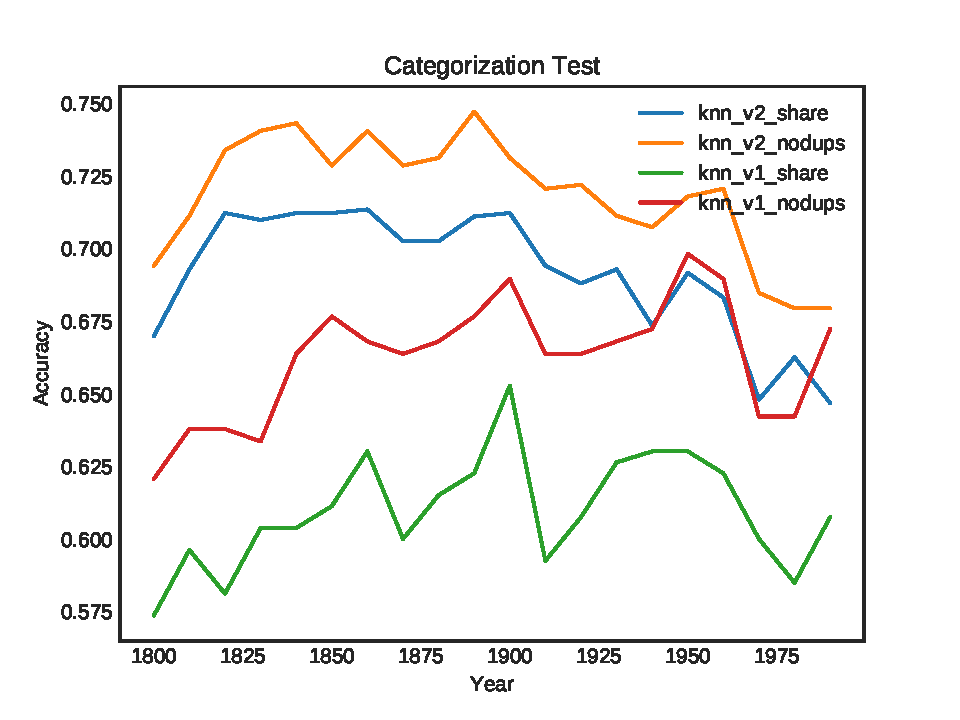
\includegraphics[width=1.3\linewidth]{../../plots-2/knn/results_categorization_test.pdf}
\end{figure}

\begin{figure}[H]
    \centerfloat
    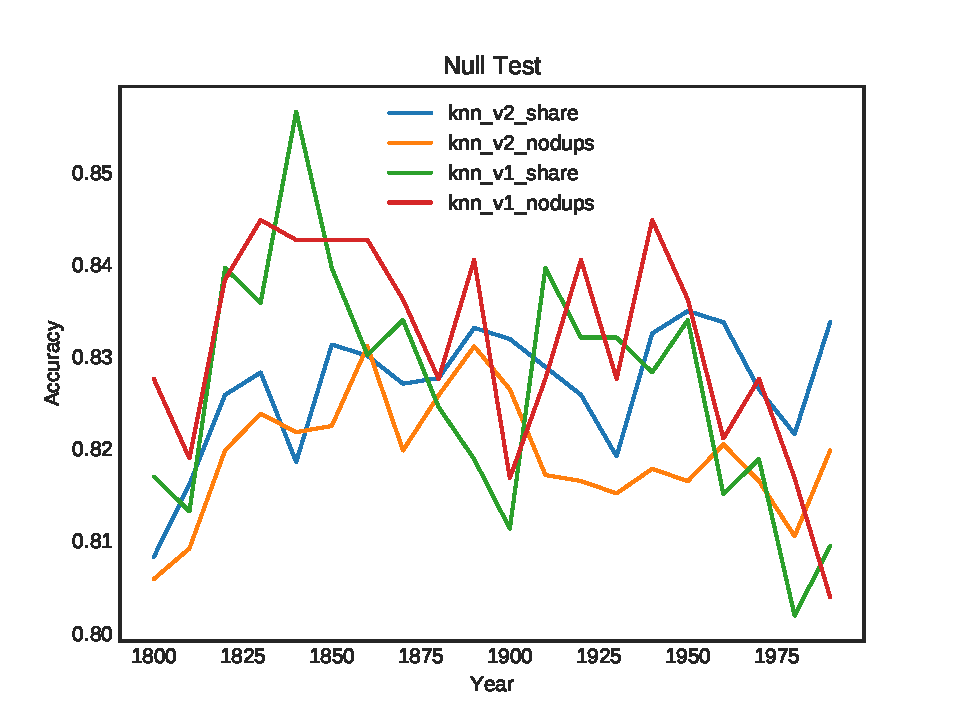
\includegraphics[width=1.3\linewidth]{../../plots-2/knn/results_null_test.pdf}
\end{figure}

\begin{figure}[H]
    \centerfloat
    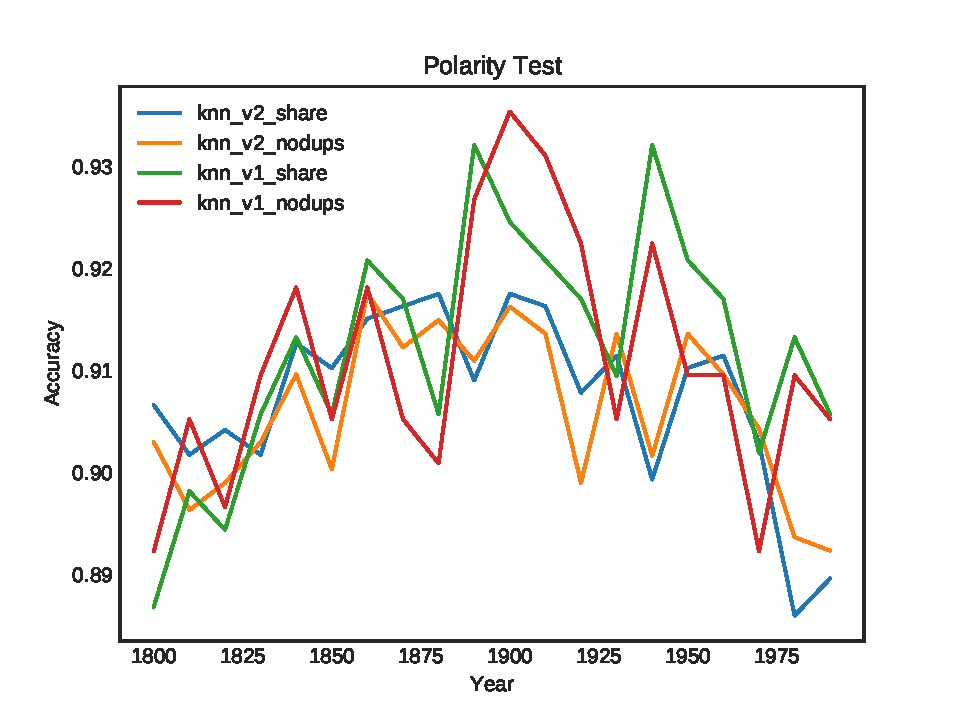
\includegraphics[width=1.3\linewidth]{../../plots-2/knn/results_polarity_test.pdf}
\end{figure}

\begin{figure}[H]
    \centerfloat
    \caption{Categorization confusion matrix: Centroid, V1, 'share'}
    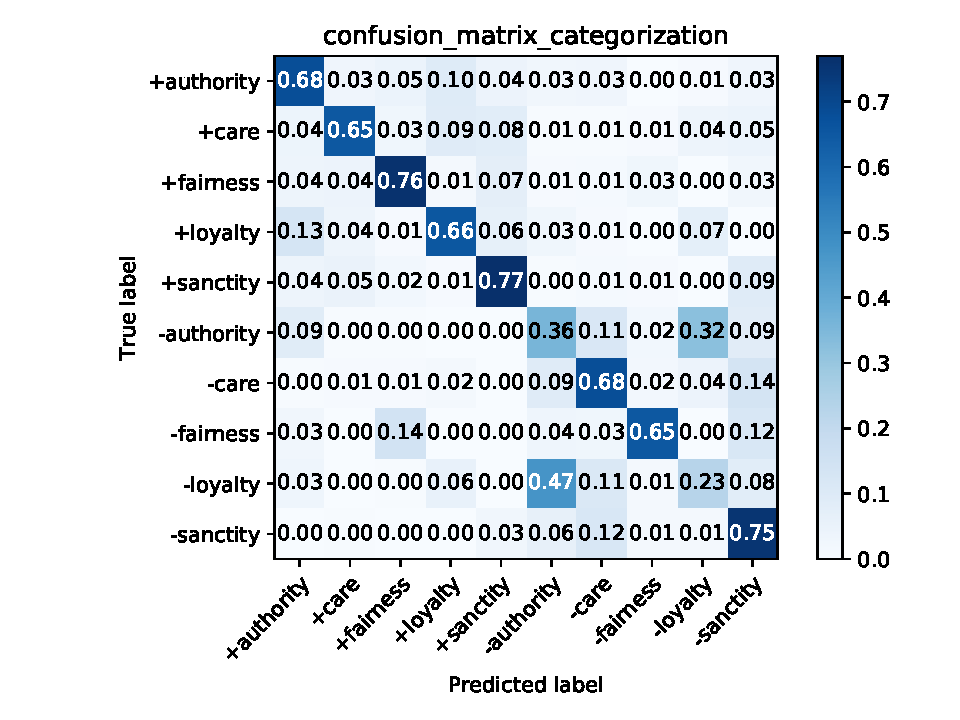
\includegraphics[width=1.3\linewidth]{../../plots-2/confusion-matrix-centroid-v1-share/confusion_matrix_categorization.pdf}
\end{figure}

\begin{figure}[H]
    \centerfloat
    \caption{Categorization confusion matrix: Centroid, V1, 'nodups'}
    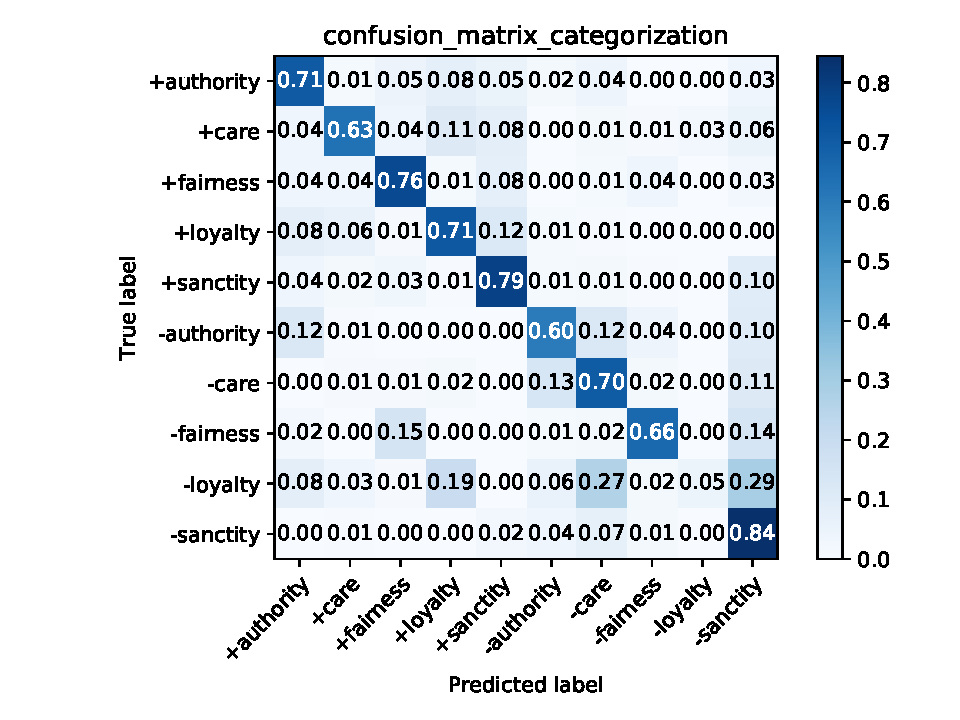
\includegraphics[width=1.3\linewidth]{../../plots-2/confusion-matrix-centroid-v1-nodups/confusion_matrix_categorization.pdf}
\end{figure}

\begin{figure}[H]
    \centerfloat
    \caption{Categorization confusion matrix: Centroid, V2, 'share'}
    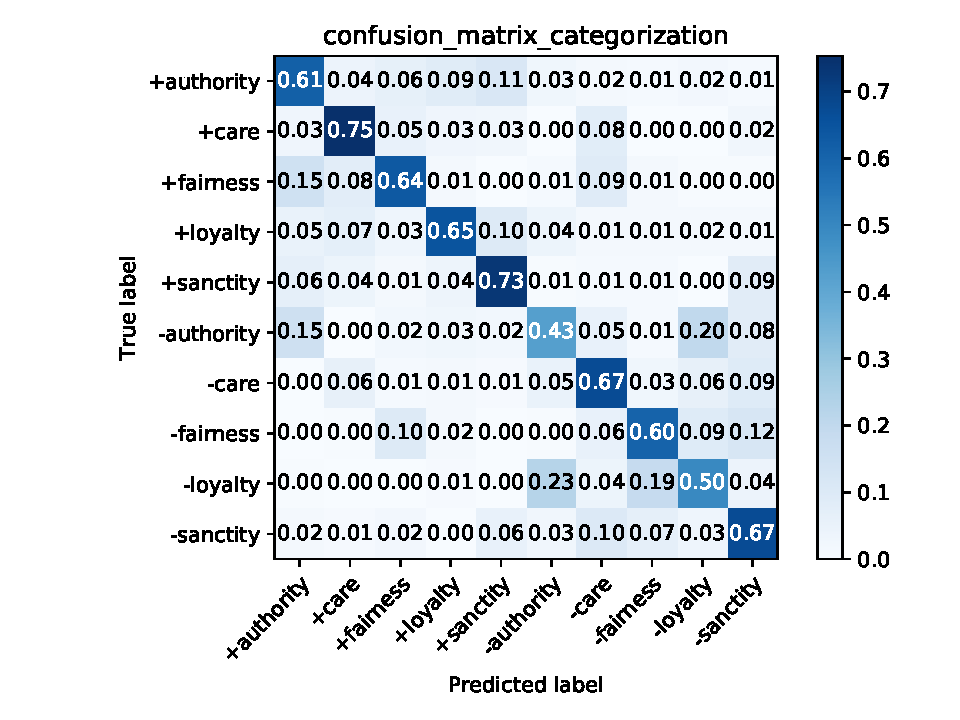
\includegraphics[width=1.3\linewidth]{../../plots-2/confusion-matrix-centroid-v2-share/confusion_matrix_categorization.pdf}
\end{figure}

\begin{figure}[H]
    \centerfloat
    \caption{Categorization confusion matrix: Centroid, V2, 'nodups'}
    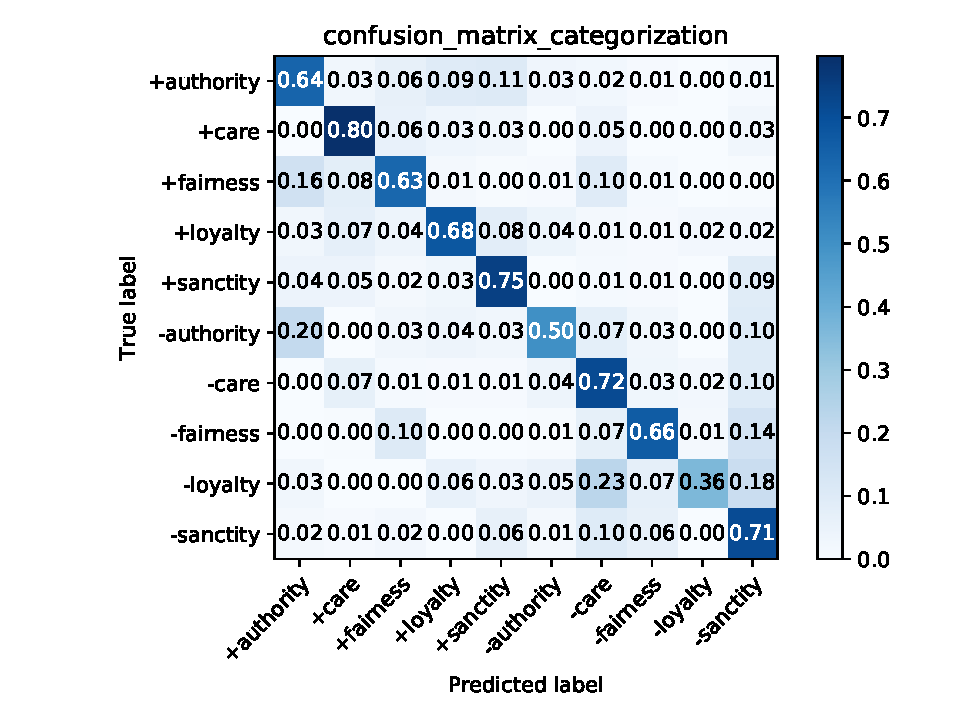
\includegraphics[width=1.3\linewidth]{../../plots-2/confusion-matrix-centroid-v2-nodups/confusion_matrix_categorization.pdf}
\end{figure}

\begin{figure}[H]
    \centerfloat
    \caption{Categorization confusion matrix: kNN, V1, 'share'}
    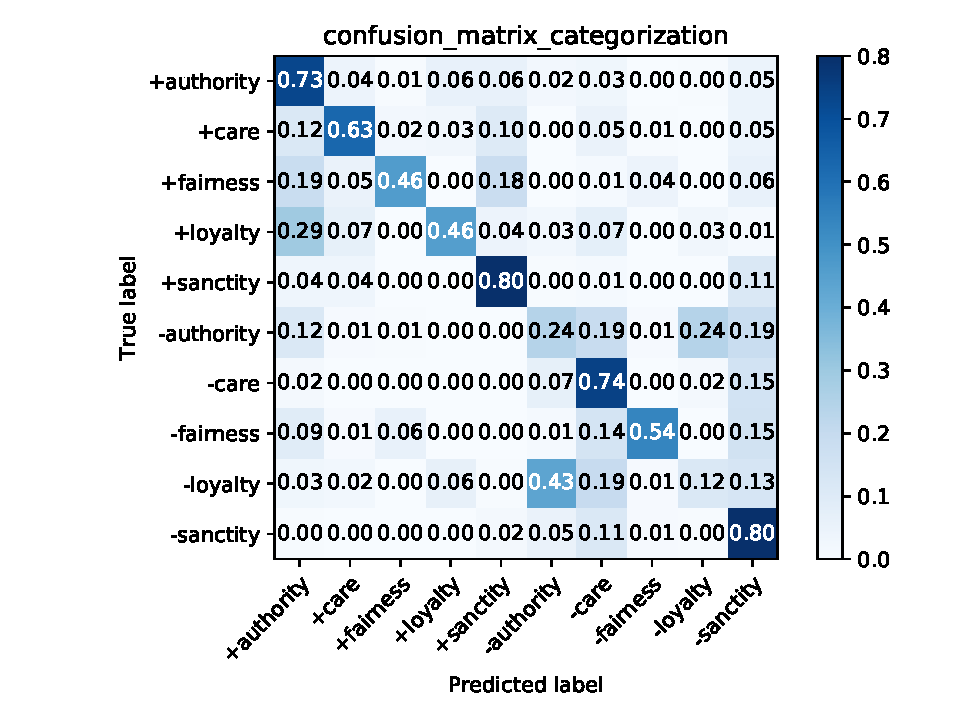
\includegraphics[width=1.3\linewidth]{../../plots-2/confusion-matrix-knn-v1-share/confusion_matrix_categorization.pdf}
\end{figure}

\begin{figure}[H]
    \centerfloat
    \caption{Categorization confusion matrix: kNN, V1, 'nodups'}
    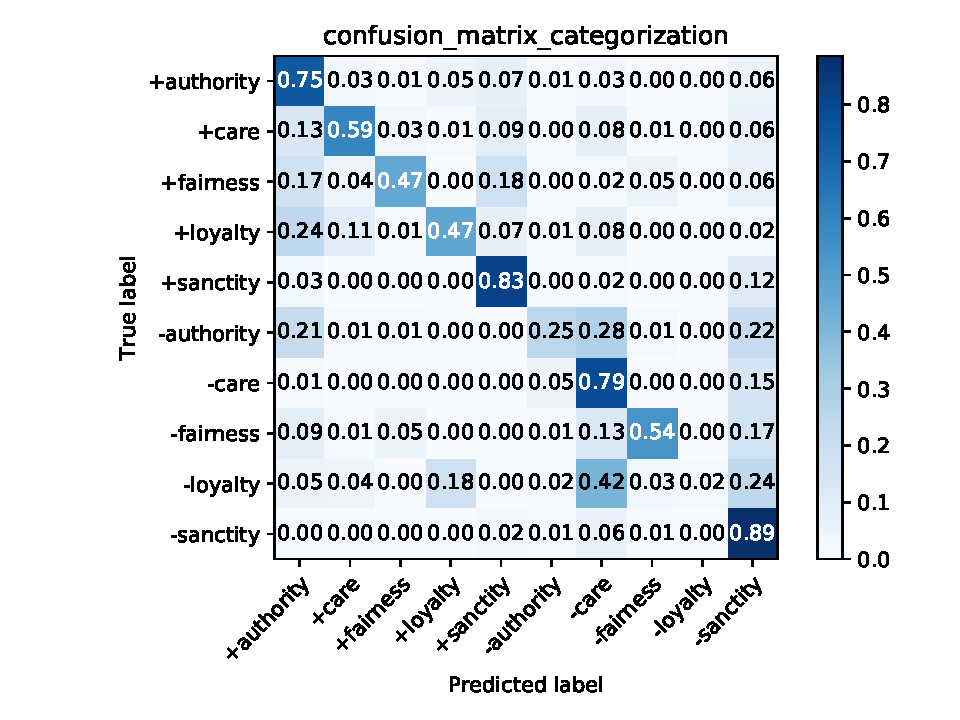
\includegraphics[width=1.3\linewidth]{../../plots-2/confusion-matrix-knn-v1-nodups/confusion_matrix_categorization.pdf}
\end{figure}

\begin{figure}[H]
    \centerfloat
    \caption{Categorization confusion matrix: kNN, V2, 'share'}
    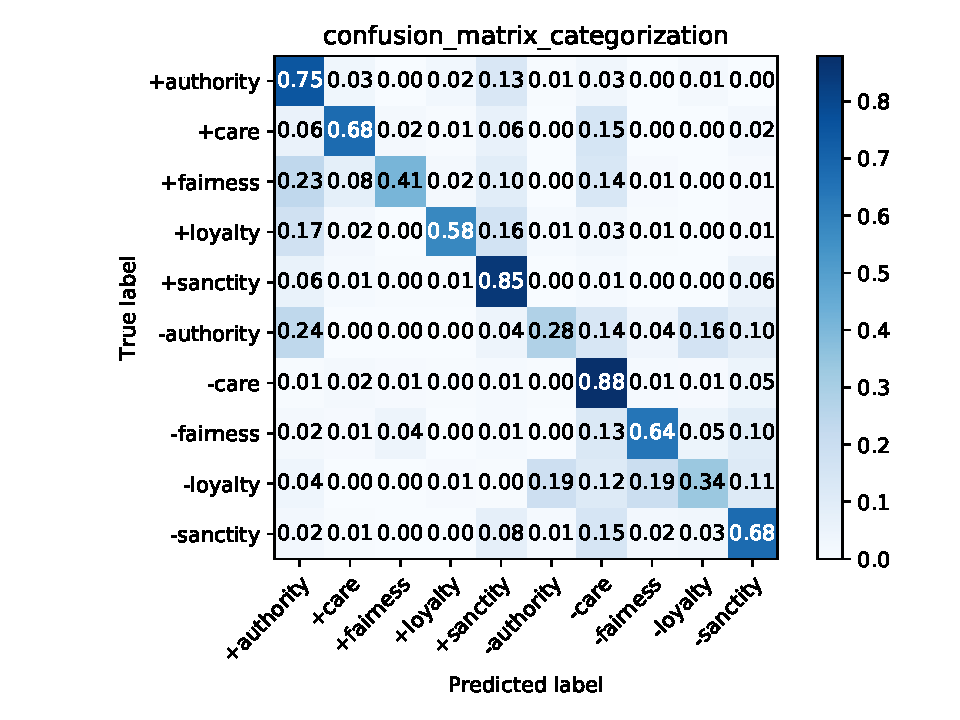
\includegraphics[width=1.3\linewidth]{../../plots-2/confusion-matrix-knn-v2-share/confusion_matrix_categorization.pdf}
\end{figure}

\begin{figure}[H]
    \centerfloat
    \caption{Categorization confusion matrix: kNN, V2, 'nodups'}
    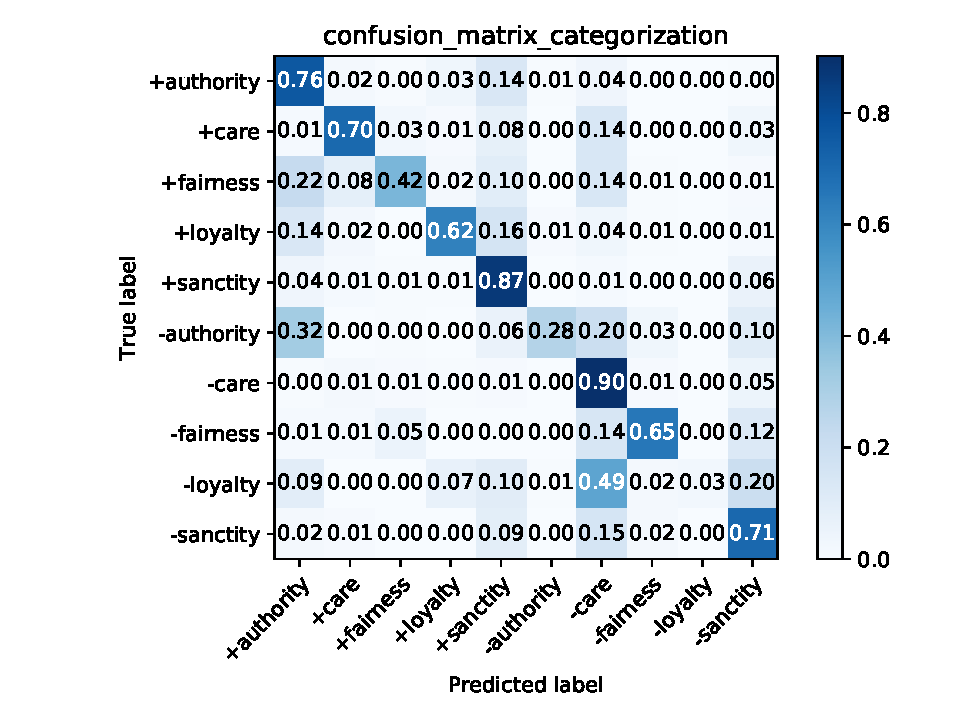
\includegraphics[width=1.3\linewidth]{../../plots-2/confusion-matrix-knn-v2-nodups/confusion_matrix_categorization.pdf}
\end{figure}

\end{document}
